\subsection{Latensi Disk}
\label{sec:latensi-disk}

Latensi \textit{disk} adalah latensi yang terjadi ketika mengakses perangkat penyimpanan seperti \textit{hard disk drive} (HDD) atau \textit{solid state drive} (SSD). Sistem penyimpanan memiliki perbedaan waktu yang jauh lebih lambat dibandingkan waktu akses dari modul memori utama \parencite{ng1991improving}.

\begin{figure}[ht]
  \centering
  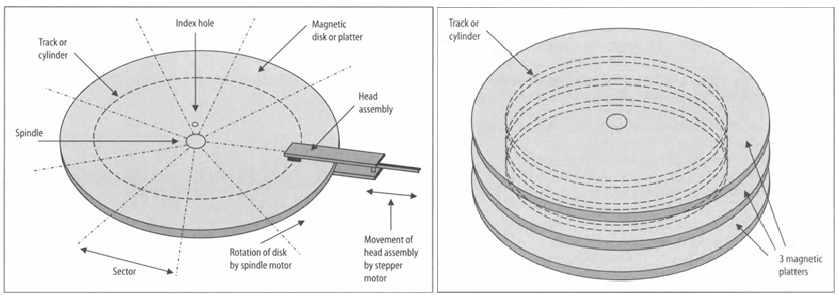
\includegraphics[width=0.95\textwidth]{resources/chapter-2/disk-structure.png}
  \caption{Struktur HDD \parencite{sammes2000disk}}
  \label{fig:hdd-structure}
\end{figure}


HDD terdiri atas susunan piringan dan penunjuk seperti yang diilustrasikan pada Gambar \ref{fig:hdd-structure}. Untuk mengakses data, pertama kali HDD harus membenarkan posisi dari kepala penunjuk sampai berada pada \textit{track} yang sesuai, waktu yang diperlukan untuk melakukan hal ini disebut dengan \textit{seek time}. Setelah kepala penunjuk sudah ada pada posisi, piringan harus berputar sampai sektor yang diperlukan berselarasan dengan kepala penunjuk tersebut, waktu ini disebut dengan \textit{rotational latency}. Karena piringan berputar terus menerus, waktu yang dibutuhkan untuk mencapai sektor yang benar bergantung pada kecepatan dari piringan tersebut. Kecepatan ini diukur menggunakan satuan \textit{rotations per minute} (RPM). Pemindahan data baru dapat dilakukan setelah kepala ada pada posisi sektor yang benar. Jika data tidak bersifat kontinu atau tersebar pada sektor yang berbeda-beda, penyesuaian kepala penunjuk dapat menyebabkan penambahan \textit{seek time} dan \textit{rotational latency} sesuai lokasi sektor tersebut. Pelaksanaan \textit{request} juga ditentukan oleh algoritma \textit{disk scheduling} yang digunakan \parencite{arpaci2018operating}.

Teknologi lain yang digunakan sebagai sistem penyimpanan adalah \textit{solid-state drive} (SSD). SSD tidak memiliki bagian mekanikal layaknya HDD, tetapi dibuat dari transistor seperti memori dan prosesor. Latensi dari SSD yang menggunakan teknologi \textit{flash} tidak lagi terpengaruh oleh peletakan data pada modul. Latensi berasal dari waktu yang digunakan oleh \textit{controller}. Hal yang dilakukan oleh \textit{controller} antara lain memetakan data pada blok, memanfaatkan \textit{cache} pada SSD, melakukan \textit{wear-leveling} untuk menyebar penggunaan block agar modul bertahan lebih lama, dan membersihkan dari blok yang sudah tidak terpakai. Dibandingkan dengan HDD, SSD memiliki kinerja yang jauh lebih baik dengan \textit{throughput} yang lebih tinggi dan latensi yang lebih rendah \parencite{arpaci2018operating}.
